\documentclass[11pt]{article}
\usepackage[utf8]{inputenc}
\usepackage{graphicx}
\usepackage[space,extendedchars]{grffile} % robust graphics paths with spaces/parentheses
\usepackage{float}
\usepackage{hyperref}
\usepackage{geometry}
\usepackage{booktabs}
\usepackage{subcaption}
\usepackage{xcolor}
\usepackage{fancyhdr}
\usepackage{titlesec}
\usepackage{enumitem}
\usepackage{amsmath}
\usepackage{microtype}

% Slightly relax line breaking to avoid overfull boxes in long lines
\emergencystretch=2em

\geometry{margin=1in, top=1.2in, bottom=1.2in}

% Image search paths (handles directories with spaces)
\graphicspath{{./figures/}{../JupyterOutputs/}{../JupyterOutputs/Classification (Final)/}{../JupyterOutputs/Classification (Tuning)/}{../JupyterOutputs/VisualizationPreprocessing/}{../JupyterOutputs/PatternAnalysis/Diagnostics/}}

% Header and footer
\pagestyle{fancy}
\fancyhf{}
\fancyhead[L]{Crime Analyzer}
\fancyhead[R]{User Guide}
\fancyfoot[C]{\thepage}
% Ensure enough space for the header to avoid warnings
\setlength{\headheight}{14pt}

% Section formatting
\titleformat{\section}{\Large\bfseries\color{black}}{\thesection}{1em}{}
\titleformat{\subsection}{\large\bfseries}{\thesubsection}{1em}{}

% Hyperlink setup
\hypersetup{
    colorlinks=true,
    linkcolor=black,
    filecolor=magenta,
    urlcolor=cyan,
    citecolor=green!50!black
}

\title{\Huge\textbf{Crime Analyzer}\\
       \Large\textit{User Guide for Tourist Safety Application}}
\author{Ferdinando Muraca, Carlo Vincenzo Stanzione}
\date{\today}

\begin{document}

\maketitle
\tableofcontents
\newpage

\section{Executive Summary}

\subsection{System Overview}
The Crime Analyzer is an intelligent system designed to assess criminal risk for tourists in New York City. By analyzing historical crime data from the NYPD with advanced techniques, the system provides a clear risk assessment (High Risk or Low Risk), a confidence score for its prediction, and an explanation of the factors contributing to the assessment.

\subsection{Key Capabilities}
\begin{itemize}[leftmargin=*]
\item Real-time safety assessment based on location, time, and user profile
\item Clear explanations for each risk assessment, showing which factors are most important
\item High overall accuracy with specialized handling of high-risk scenarios
\item Analysis of crime patterns to reveal trends and associations
\end{itemize}

\subsection{Target Users}
\begin{itemize}[leftmargin=*]
\item \textbf{Tourists:} To assess personal safety and increase awareness of local risks.
\item \textbf{Individuals interested in buying or renting a home:} To check whether the address of a property is located in a safe area.
\item \textbf{Other users:} Anyone who wants to know the risk level of a specific area for personal or planning reasons.
\end{itemize}

\section{Quick Start Guide}

\subsection{Getting Started in 3 Steps}
\begin{enumerate}
\item \textbf{Provide Your Information:}
  \begin{itemize}
  \item Allow the application to access your location (GPS coordinates).
  \item Enter basic information about yourself (age group, sex, race).
  \item The system automatically uses the current time.
  \end{itemize}

\item \textbf{Receive Your Assessment:}
  \begin{itemize}
  \item The system will immediately provide a \texttt{HIGH RISK} or \texttt{LOW RISK} classification.
  \item You will also see a confidence score, indicating how certain the system is about its prediction.
  \item The key factors that influenced the result will be explained.
  \end{itemize}

\item \textbf{Make Informed Decisions:}
  \begin{itemize}
  \item Use the result as one of several factors in your safety planning.
  \item Pay special attention to predictions where the confidence is not very high (e.g., between 40\% and 60\%).
  \item Consider the local crime patterns provided with your result to better understand the context.
  \end{itemize}
\end{enumerate}

\subsection{Interpreting Your Result}
\begin{itemize}[leftmargin=*]
\item \textbf{LOW RISK:} Historical data suggests favorable conditions. However, it is always important to follow common safety practices.
\item \textbf{HIGH RISK:} The system has identified indicators of increased risk. It is advisable to prefer well-lit, populated areas and consider adjusting your travel plans.
\item \textbf{Confidence Score:} This score reflects the model's certainty. A result with low confidence should be interpreted with caution.
\item \textbf{Context Matters:} Review the trends provided to understand which factors (time, location, surroundings) are most influencing the risk.
\end{itemize}

\subsubsection*{Recommended Actions by Confidence}
\begin{center}
\begin{tabular}{@{}lll@{}}
	oprule
	extbf{Classification} & \textbf{Confidence band} & \textbf{Suggested action} \\
\midrule
LOW RISK  & 60--100\% & Proceed, remain aware of surroundings. \\
LOW RISK  & 40--60\%  & Proceed with caution; check contextual trends. \\
HIGH RISK & 60--100\% & Prefer well-lit, populated routes; consider alternatives. \\
HIGH RISK & 40--60\%  & Increase caution; avoid isolated areas; re-check later. \\
\bottomrule
\end{tabular}
\end{center}

\subsection{Example Usage Scenario}
\textbf{Scenario:} A tourist is planning an evening out and wants to assess the risk of visiting Times Square around 9 PM.
\begin{itemize}[leftmargin=*]
    \item \textbf{Input:} They provide their location (Times Square), the time (9 PM), and their personal information.
    \item \textbf{Assessment:} The system returns a \texttt{HIGH RISK} classification with a confidence score of 71\%.
    \item \textbf{Explanation:} The key contributing factors are the late hour and the high concentration of bars in the area.
    \item \textbf{Context:} The system also highlights relevant crime trends for Manhattan, such as a strong association between certain age groups and suspect profiles.
    \item \textbf{Decision:} Aware of the specific risk factors, the tourist decides to stay in more crowded and well-lit areas.
\end{itemize}

\section{How the System Works}

\subsection{System Overview}
The Crime Analyzer uses a sophisticated pipeline to deliver real-time crime risk assessments. The architecture is built to enterprise-grade standards, ensuring reliability and scalability.

\subsubsection{Core Components}
\begin{itemize}[leftmargin=*]
\item \textbf{Data Engine:} Integrates historical NYPD complaint data and enriches it with geographic and temporal features.
\item \textbf{Prediction Model:} A machine learning model that calculates the risk level based on the input data.
\item \textbf{Inference Engine:} Provides the final risk assessment and confidence score.
\item \textbf{Explainability Module:} Identifies and presents the key factors influencing the prediction.
\item \textbf{Pattern Analysis:} Discovers underlying crime trends and patterns from the data.
\end{itemize}

\subsection{Input Specification}
The system requires the following information to generate an assessment:

\subsubsection{Required Inputs}
\begin{itemize}[leftmargin=*]
\item \textbf{Geographic Coordinates:} Latitude and Longitude.
\item \textbf{User Profile:} Age Group, Race, and Sex, based on standardized categories.
\end{itemize}

\subsubsection{Derived Information}
From the user's coordinates and the current time, the system automatically generates dozens of additional data points for a more accurate analysis. These include:
\begin{itemize}[leftmargin=*]
\item \textbf{Temporal Information (e.g., Hour, Day of the Week, Season):} To understand time-based patterns.
\item \textbf{Geographic Information (e.g., Borough):} To consider location-specific trends.
\item \textbf{Points of Interest (POI):} Information about nearby bars, metro stations, schools, etc., to assess the environmental context.
\end{itemize}

\subsection{Output Specification}
The system provides a clear and concise output for each assessment:
\begin{itemize}[leftmargin=*]
\item \textbf{Primary Output:} A binary classification of \texttt{HIGH RISK} or \texttt{LOW RISK}.
\item \textbf{Confidence Score:} A percentage indicating the model's confidence in its prediction for the \texttt{HIGH RISK} class.
\item \textbf{Contextual Trends:} The system enriches the response with relevant crime patterns for the specific time and location, helping the user understand the broader context.
\end{itemize}

\section{Data and Analysis}

\subsection{Data Sources}
The system is built on a foundation of reliable and comprehensive data to ensure the quality of its assessments.

\subsubsection{Primary Data Sources}
\begin{itemize}[leftmargin=*]
\item \textbf{NYPD Complaint Data:} Historical and current crime reports from the New York City Police Department.
\item \textbf{Geographic Data:} Information on Points of Interest, such as transit stations, commercial establishments, and schools.
\end{itemize}

\subsection{Data Processing}
To ensure accuracy, the raw data undergoes a rigorous preparation process. This includes cleaning the data, handling missing values, and integrating information from different sources. This preparation is crucial for the model to learn effectively and make reliable predictions.

\section{Model Performance}
The Crime Analyzer's prediction model was chosen after extensive testing and comparison with over 15 other algorithms. The final model demonstrates a strong balance of performance, reliability, and interpretability.

\subsection{Performance Highlights}
On a hold-out test set, the model achieved:
\begin{itemize}[leftmargin=*]
\item \textbf{96.5\% Accuracy:} The model is highly accurate in its overall predictions.
\item \textbf{Strong Discriminative Ability:} The model is very effective at distinguishing between high-risk and low-risk situations.
\item \textbf{Balanced Performance:} While no model is perfect, this system is tuned to provide a practical balance between identifying potential risks and avoiding excessive false alarms.
\end{itemize}

\subsection{Model Validation}
The model's performance has been rigorously tested to ensure it is both stable and reliable. It has been validated to perform consistently across different data samples, which indicates that it can generalize well to new, unseen situations. This robustness is critical for a system designed for real-world use.

\subsection{Illustrative Outputs}
\begin{figure}[H]
  \centering
  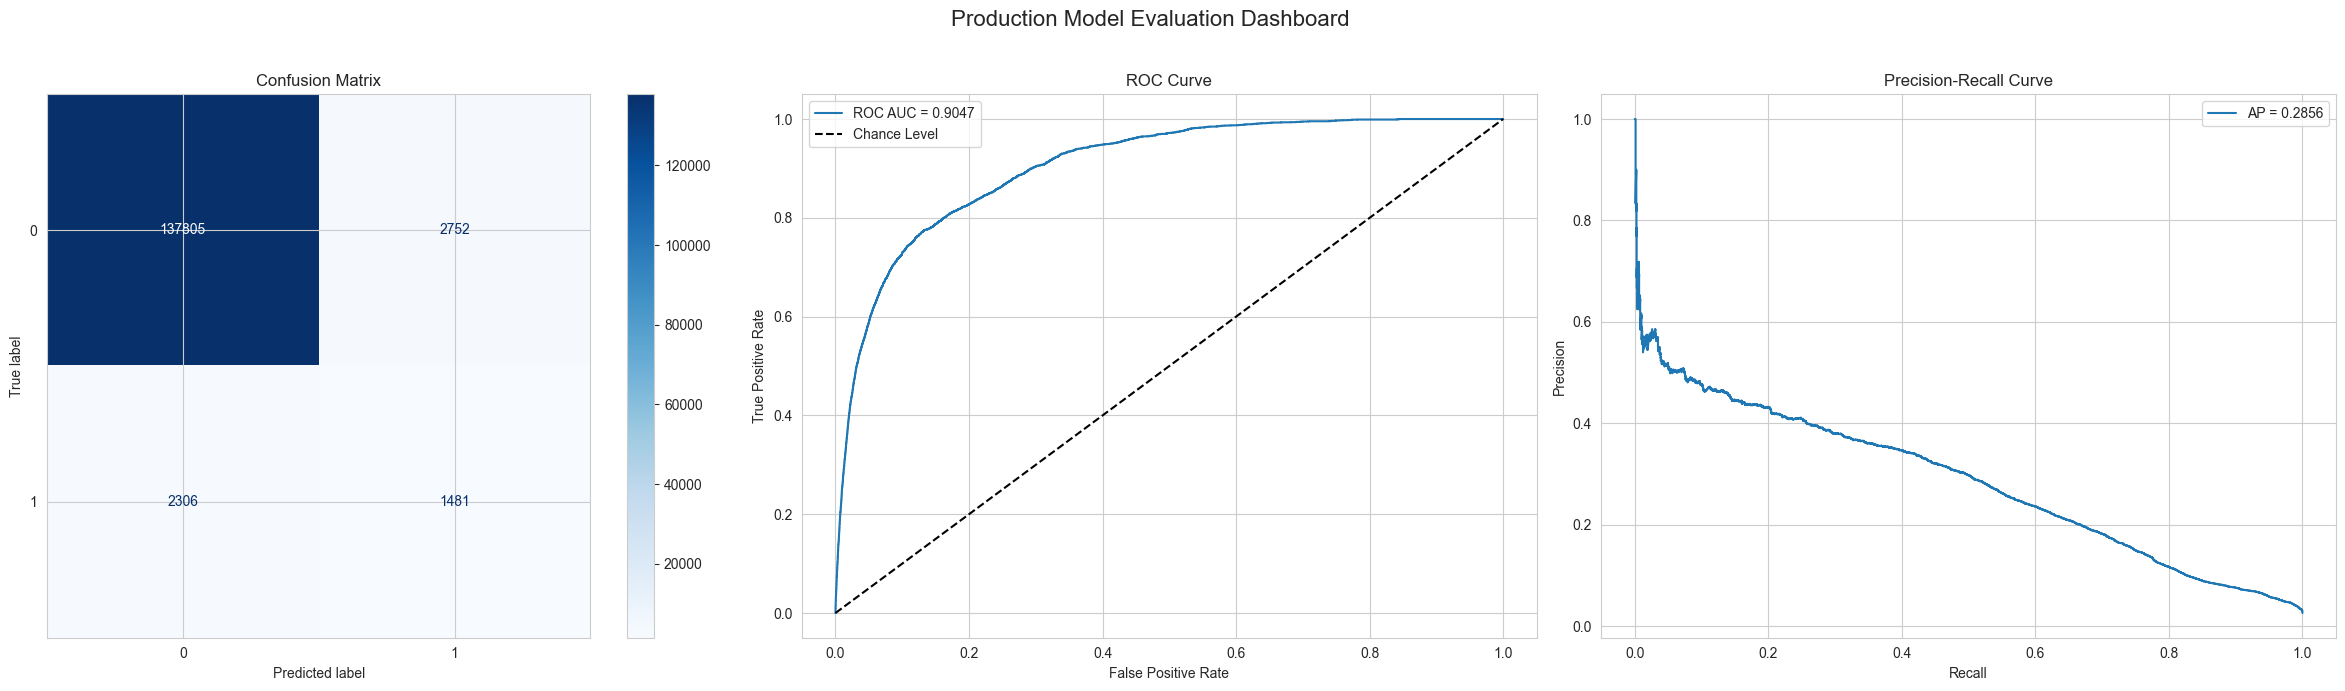
\includegraphics[width=0.98\textwidth]{LogisticRegression_evaluation_dashboard.png}
  \caption{Model evaluation overview on the hold-out set.}
\end{figure}

\begin{figure}[H]
  \centering
  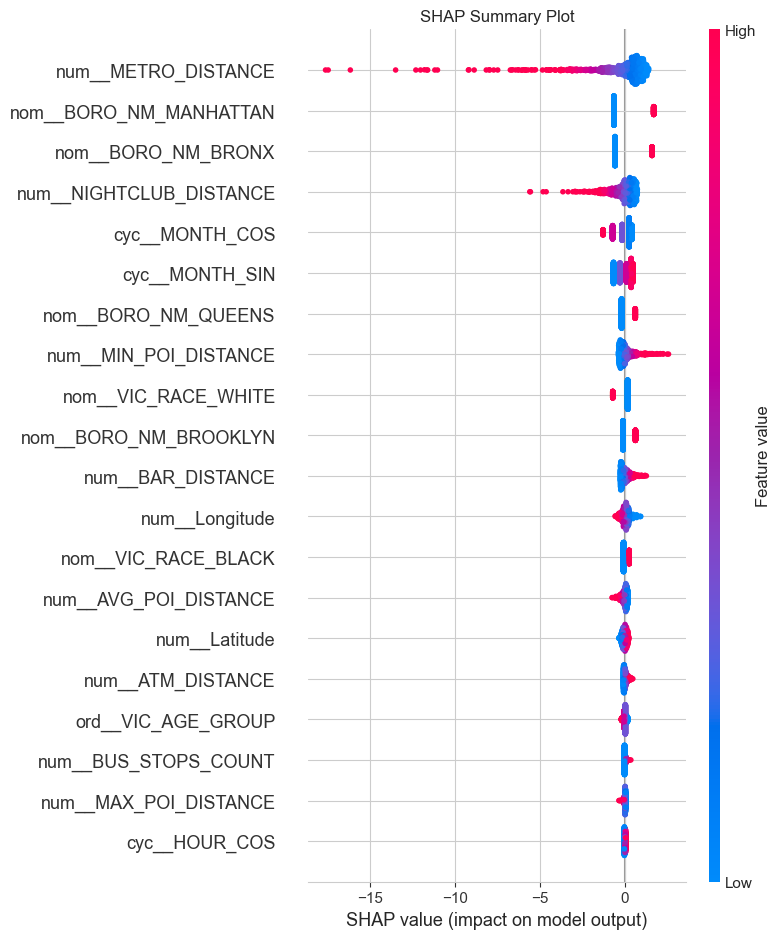
\includegraphics[width=0.9\textwidth]{LogisticRegression_shap_summary.png}
  \caption{Explainability summary highlighting feature contributions (SHAP).}
\end{figure}

\section{Understanding the Predictions}
Explainability is a core principle of the Crime Analyzer. The system is designed not only to provide an assessment but also to explain the "why" behind it.

\subsection{Explainable Predictions}
For every prediction, the system identifies the key factors that influenced the outcome. For example, it might highlight that the time of day or the proximity to a certain type of location was a major contributor to a "High Risk" assessment. This helps users understand the context of their situation and make more informed decisions.

\subsection{Pattern Analysis}
In addition to individual predictions, the system analyzes the data to uncover broader crime patterns and trends. For instance, it might identify that certain types of crime are more common in specific boroughs or at particular times of the day. These insights are provided alongside the risk assessment to give users a more complete picture of the safety landscape.

\vspace{0.5em}
\noindent\textit{Example insight (Evening time bucket):}
\begin{verbatim}
--- Top-K Rules for TimeBucket = EVENING (172,881 records) ---

IF (SUSP_AGE=25-44) THEN (SUSP_SEX=M)
  - Kulc: 0.624, Conf: 78.95%, Lift: 1.43, Support: 0.2538, Score: 0.314

IF (VIC_SEX=F) THEN (HAS_POI=NO)
  - Kulc: 0.563, Conf: 74.27%, Lift: 1.14, Support: 0.2495, Score: 0.281

IF (LAW_CAT=FELONY) THEN (HAS_POI=NO)
  - Kulc: 0.505, Conf: 66.66%, Lift: 1.03, Support: 0.2227, Score: 0.238
\end{verbatim}

\subsection{Glossary}
\begin{itemize}[leftmargin=*]
  \item \textbf{Confidence score:} Model-estimated probability for the \texttt{HIGH RISK} class.
  \item \textbf{POI:} Points of Interest (e.g., bars, schools, transit stops) near a location.
  \item \textbf{SHAP:} A method to attribute each feature's contribution to a specific prediction.
\end{itemize}

\section{Responsible Use and Ethics}
\begin{itemize}[leftmargin=*]
\item \textbf{Fairness awareness:} Inputs like age group, sex, and race mirror categories in source data and are used to reflect observed patterns, not to ascribe individual traits. Historical data can encode societal biases; interpret outputs accordingly.
\item \textbf{Appropriate use:} The tool supports personal safety awareness for civilians and planners. It is not intended for law enforcement decision-making about individuals.
\item \textbf{Transparency:} Explanations are surfaced to help users understand drivers of the assessment.
\item \textbf{Human judgment:} Always complement outputs with local knowledge and situational awareness.
\end{itemize}

\section{System Limitations}
It is important to understand the limitations of the Crime Analyzer to use it effectively and responsibly.

\subsection{Known Constraints}
\begin{itemize}[leftmargin=*]
\item \textbf{Based on Historical Data:} The model's predictions are based on past crime data and may not reflect sudden, real-time events.
\item \textbf{Data Gaps:} The system may be less effective in areas with limited historical crime data.
\item \textbf{Not a Crystal Ball:} The predictions are probabilistic estimates, not guarantees of future outcomes.
\end{itemize}

\subsection{Risk Mitigation}
To ensure responsible use, the system is designed with several safeguards:
\begin{itemize}[leftmargin=*]
\item \textbf{Regular Updates:} The model is periodically retrained with the latest data to keep its knowledge current.
\item \textbf{Clear Communication:} The system's limitations are clearly communicated to users.
\item \textbf{User Discretion Advised:} Users are encouraged to use the assessment as one of many tools in their decision-making process and to always remain aware of their surroundings.
\end{itemize}

\section{FAQ}
\begin{enumerate}[leftmargin=*]
  \item \textbf{Does a \texttt{LOW RISK} result mean I'm safe?} No. It indicates favorable conditions historically, not a guarantee.
  \item \textbf{Why is the confidence sometimes around 50\%?} Inputs may be ambiguous or the situation similar to both classes; treat with extra caution.
  \item \textbf{Do you track my identity?} The system uses the inputs you provide to compute the assessment. Data handling follows the deployment's privacy policy.
  \item \textbf{Can I use this for cities other than NYC?} This version is trained on NYC data; broader coverage is in the roadmap.
  \item \textbf{What if the result seems off?} Re-check location accuracy, time, and inputs; review contextual trends and act conservatively.
\end{enumerate}

\section{Future Enhancements}
The Crime Analyzer is committed to continuous improvement. Future plans include:
\begin{itemize}[leftmargin=*]
\item \textbf{Enhanced Features:} Incorporating more sophisticated data, such as real-time event information.
\item \textbf{Interactive Visualizations:} Developing web-based maps to explore risk areas interactively.
\item \textbf{Expansion:} Adapting the system for use in other major cities.
\end{itemize}

\section{Conclusion}
The Crime Analyzer is a powerful tool for enhancing personal safety. By providing accurate, explainable, and context-aware risk assessments, it empowers users to make smarter, safer decisions. Its applications extend beyond tourism to urban planning, law enforcement, and other areas where data-driven insights can contribute to a safer society.


\end{document}